\subsection{Eksperimentų orkestracija (\texttt{main.py})}
\label{subsec:main_orchestration}

Failas \texttt{main.py} sujungia visas pirmiau aprašytas klases į vientisą eksperimentų vykdymo procesą: užkrauna duomenis, paleidžia penkis tyrimus, paskaičiuoja kiekvieno modelio metrikas ir parenka geriausią modelį testavimui (žr.~\ref{fig:main_first} – \ref{ref:main_last} pav.).

\begin{figure}[H]
    \centering
    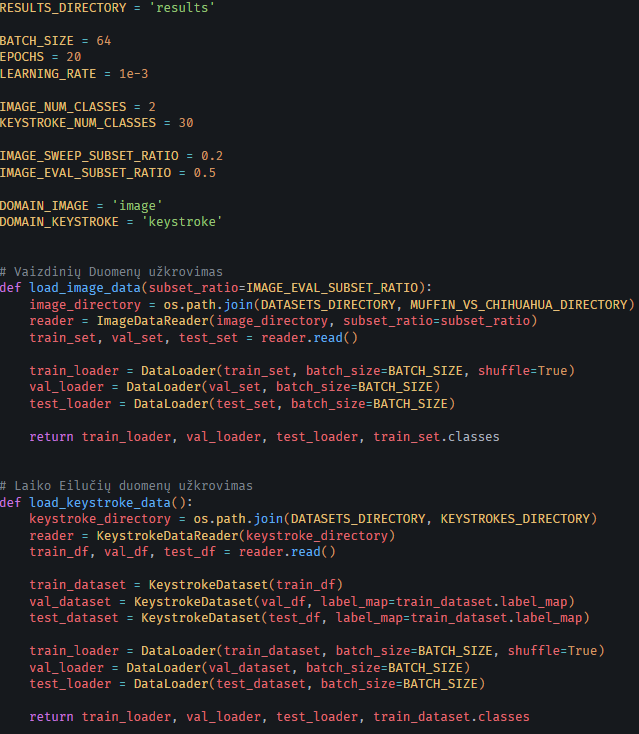
\includegraphics[width=0.85\linewidth]{3Lab/overleaf/images/main_1.png}
    \caption{Eksperimentų orkestracijos kodas I dalis.}
    \label{fig:main_first}
\end{figure}

\begin{figure}[H]
    \centering
    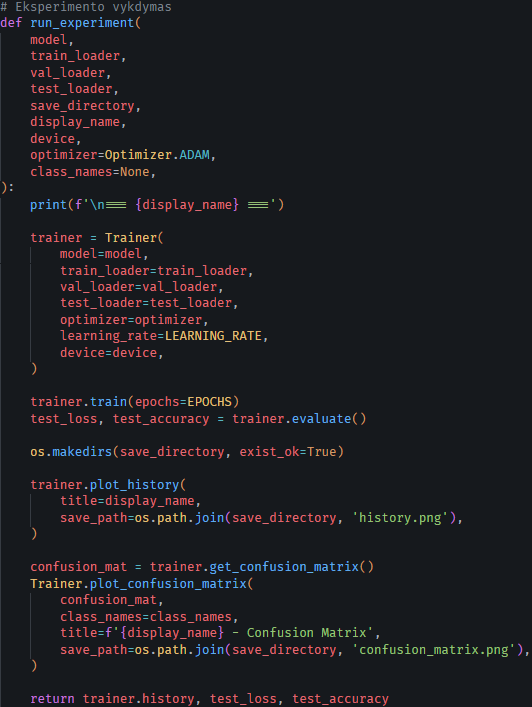
\includegraphics[width=0.85\linewidth]{3Lab/overleaf/images/main_2.png}
    \caption{Eksperimentų orkestracijos kodas II dalis.}
    \label{fig:main_second}
\end{figure}

\begin{figure}[H]
    \centering
    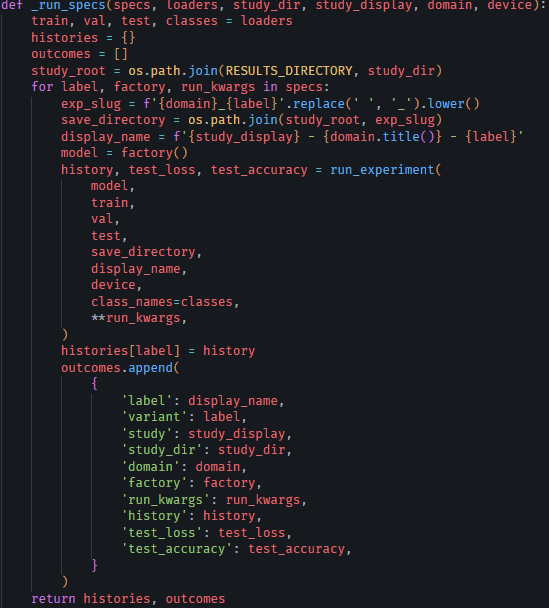
\includegraphics[width=0.85\linewidth]{3Lab/overleaf/images/main_3.png}
    \caption{Eksperimentų orkestracijos kodas III dalis.}
    \label{fig:main_third}
\end{figure}

\begin{figure}[H]
    \centering
    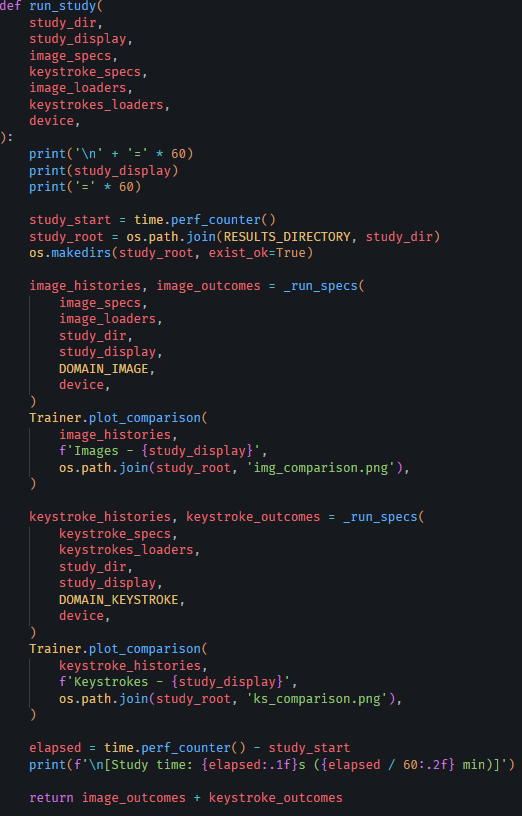
\includegraphics[width=0.85\linewidth]{3Lab/overleaf/images/main_4.png}
    \caption{Eksperimentų orkestracijos kodas IV dalis.}
    \label{fig:main_fourth}
\end{figure}

\begin{figure}[H]
    \centering
    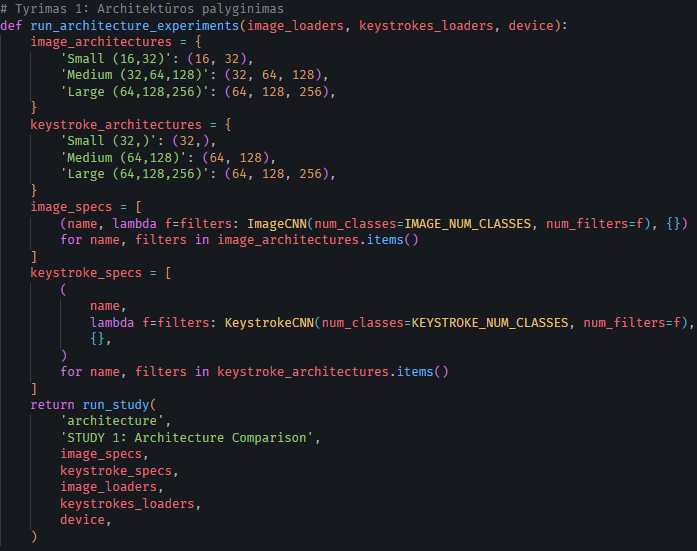
\includegraphics[width=0.85\linewidth]{3Lab/overleaf/images/main_5.png}
    \caption{Eksperimentų orkestracijos kodas V dalis.}
    \label{fig:main_fifth}
\end{figure}

\begin{figure}[H]
    \centering
    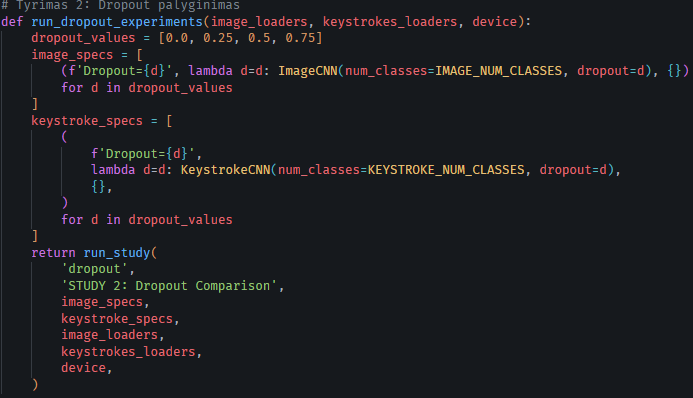
\includegraphics[width=0.85\linewidth]{3Lab/overleaf/images/main_6.png}
    \caption{Eksperimentų orkestracijos kodas VI dalis.}
    \label{fig:main_sixth}
\end{figure}

\begin{figure}[H]
    \centering
    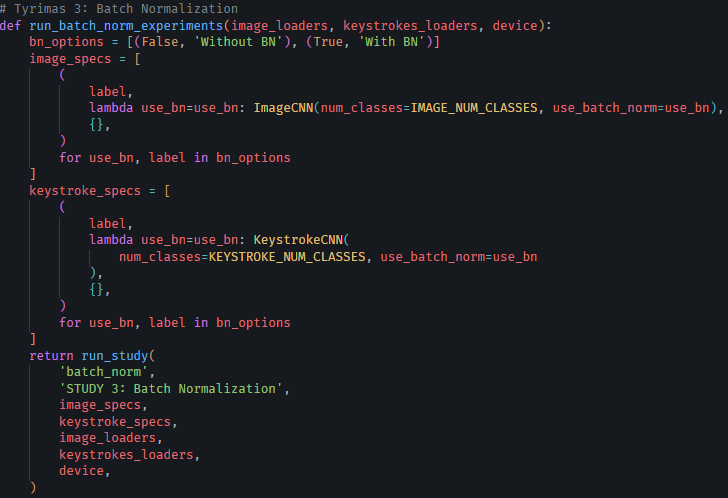
\includegraphics[width=0.85\linewidth]{3Lab/overleaf/images/main_7.png}
    \caption{Eksperimentų orkestracijos kodas VII dalis.}
    \label{fig:main_seventh}
\end{figure}

\begin{figure}[H]
    \centering
    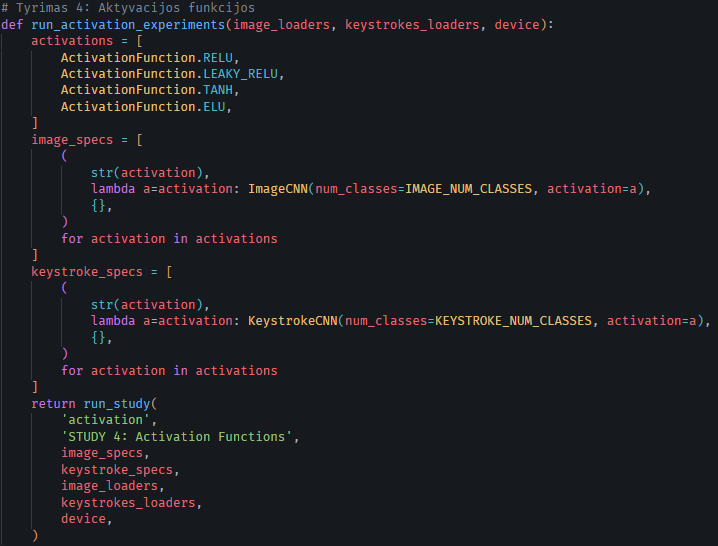
\includegraphics[width=0.85\linewidth]{3Lab/overleaf/images/main_8.png}
    \caption{Eksperimentų orkestracijos kodas VIII dalis.}
    \label{fig:main_eighth}
\end{figure}

\begin{figure}[H]
    \centering
    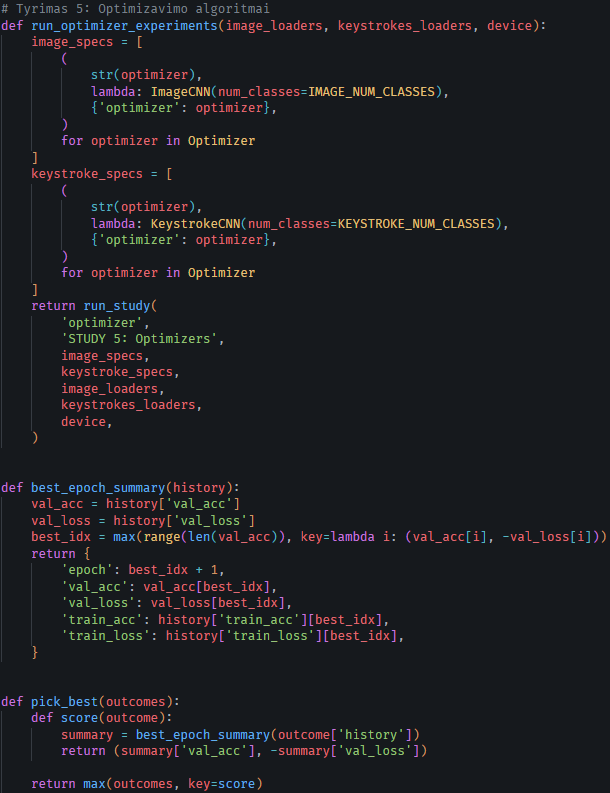
\includegraphics[width=0.85\linewidth]{3Lab/overleaf/images/main_9.png}
    \caption{Eksperimentų orkestracijos kodas IX dalis.}
    \label{fig:main_ninth}
\end{figure}

\begin{figure}[H]
    \centering
    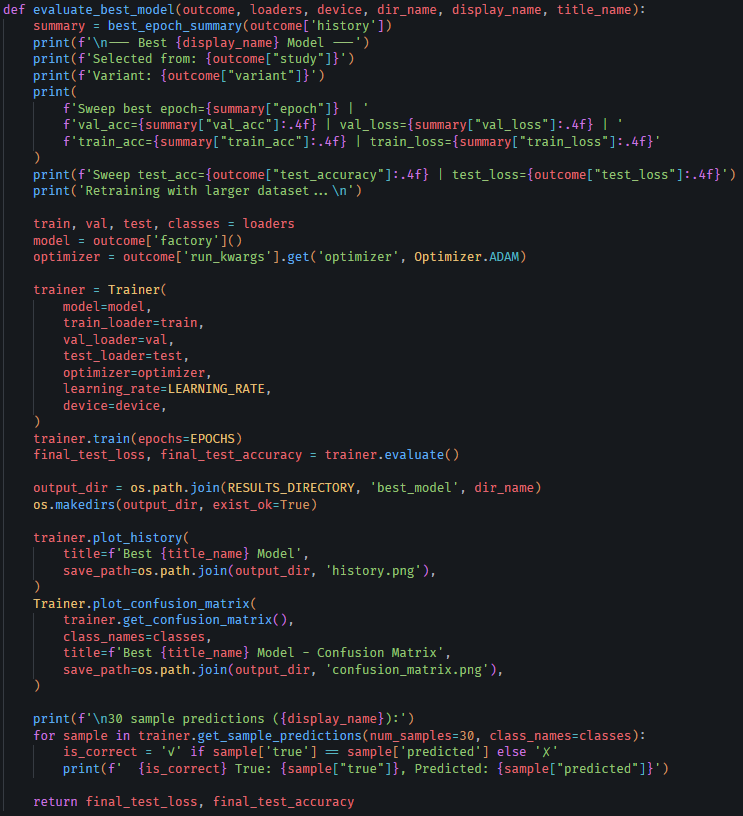
\includegraphics[width=0.85\linewidth]{3Lab/overleaf/images/main_10.png}
    \caption{Eksperimentų orkestracijos kodas X dalis.}
    \label{fig:main_10}
\end{figure}

\begin{figure}[H]
    \centering
    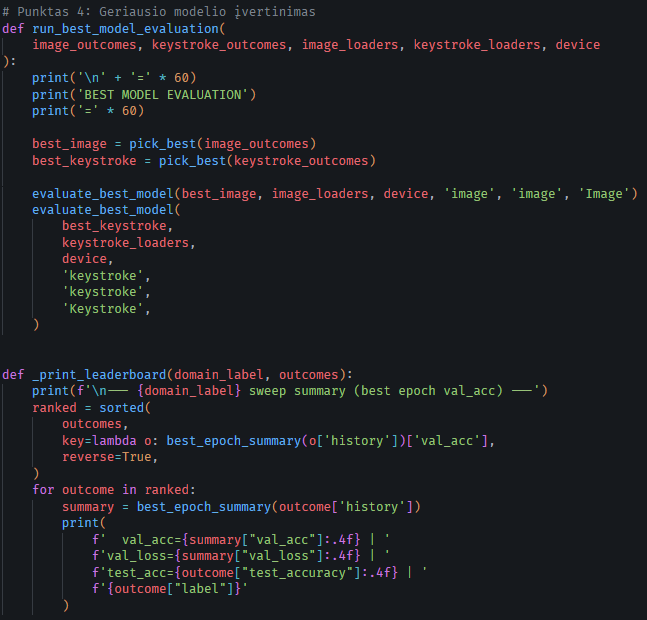
\includegraphics[width=0.85\linewidth]{3Lab/overleaf/images/main_11.png}
    \caption{Eksperimentų orkestracijos kodas XI dalis.}
    \label{fig:main_last}
\end{figure}

Pagrindinės funkcijos:
\begin{itemize}
    \item \texttt{load\_image\_data} ir \texttt{load\_keystroke\_data} – sukuria \texttt{DataLoader} objektus visoms trims aibėms; vaizdams perduoda \texttt{subset\_ratio} parametrą.
    \item \texttt{run\_experiment} – sukuria \texttt{Trainer}, paleidžia mokymą $20$ epochų, įvertina ant testavimo aibės ir išsaugo istorijos bei klasifikavimo matricos paveikslėlius.
    \item \texttt{run\_study} – paleidžia visus eksperimentus, priklausančius vienam tyrimui, ir sugeneruoja palyginimo grafiką (\textit{val\_loss} ir \textit{val\_acc} priklausomybės nuo epochos).
    \item \texttt{run\_architecture\_experiments}, \texttt{run\_dropout\_experiments}, \texttt{run\_batch\_norm\_experiments}, \texttt{run\_activation\_experiments}, \texttt{run\_optimizer\_experiments} – penki tyrimai, atitinkantys užduoties reikalavimus (žr.~\ref{sec:tyrimo_rezultatai} sk.).
    \item \texttt{pick\_best} – iš visų $17$ eksperimentų variantų atrenka geriausią pagal didžiausią validavimo tikslumą ir mažiausią validavimo paklaidą (lygiosioms taikomas leksikografinis kriterijus).
    \item \texttt{evaluate\_best\_model} – iš naujo apmoko geriausią konfigūraciją su didesniu vaizdų poaibiu (\texttt{subset\_ratio}~$=0{,}5$), išsaugo galutines istorijos ir klasifikavimo matricos vizualizacijas, atspausdina $30$ testinių pavyzdžių spėjimus.
\end{itemize}
